\documentclass[../main.tex]{subfiles}
\graphicspath{{\subfix{../../images/}}}

\begin{document}

\subsection{Digital Currencies}

Digital currencies are similar to real-life \textbf{fiat currencies}, like US dollars, Singapore Dollars, Chinese Yuan, or Euros, but \textbf{they do not have any physical, tangible form}. Instead, they are only represented in digital means. However, they are typically tied to a real currenciy.

Digital currencies use a \textbf{central banking system}, where all transactions eventually go through a central entity. It can be modeled as follows:

\begin{figure}[H]
    \centering
    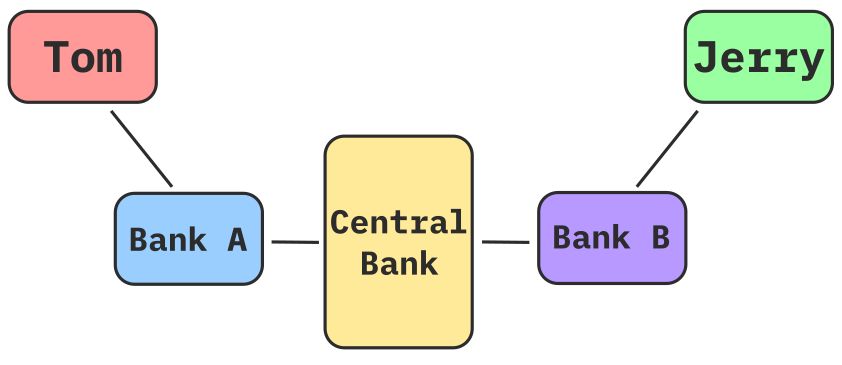
\includegraphics[width=0.8\textwidth]{centralbanksystem.png}
    \caption{How a central banking system works}
    \label{fig:centralbankingsystem}
\end{figure}

\subsubsection{Examples of digital currencies}

They include but are not limited to:

\begin{itemize}
    \item \textbf{PayNow/PayLah} in Singapore are common digital currency platforms. They are tied to the Singapore Dollar, they have no physical form, and all transactions take place digitally.
    \item \textbf{PayPal} is also a good example, a common example for international users.
    \item \textbf{WeChat Pay} is predominantly used in China and is tied to the Chinese Yuan.
\end{itemize}

\subsection{Cryptocurrencies}

Unlike digital currencies, cryptocurrencies do not operate through any central bank, instead, all the transactions are modeled through a \textbf{blockchain.}

\begin{figure}[H]
    \centering
    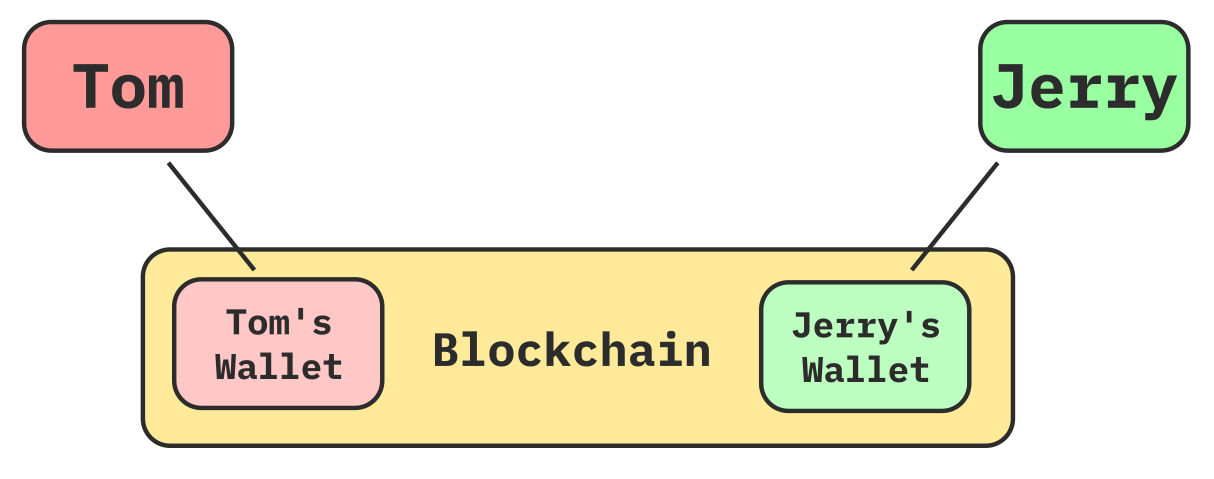
\includegraphics[width=0.7\textwidth]{cryptocurrency.png}
    \caption{How a transaction occurs on a cryptocurrency.}
    \label{fig:cryptocurrency}
\end{figure}

Figure \ref{fig:cryptocurrency} shows a mysterious "blockchain", which is actually a central part to cryptocurrencies. \textbf{Instead of physical money or digital money in the form of numbers being exchanged, the blockchain relies on the act of sending money itself.} These acts are noted down.

Therefore, when Tom wants to send Jerry 10 dollars, instead of handing him 10 dollars, he sends a message to everybody else on the blockchain, saying that he gave Jerry 10 dollars. \textbf{Everyone else acknowledges} that the money had been sent, and they note this transaction down. Since everybody has proof that the money was sent, everyone can assume Jerry now has 10 dollars in his wallet.

These notes are not actually kept on a physical ledger, however, there are put on a blockchain.

\subsubsection{Blockchains}

\begin{figure}[H]
    \centering
    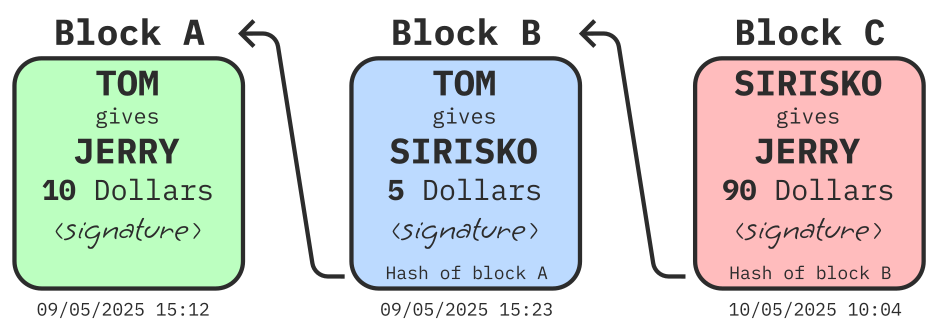
\includegraphics[width=0.85\textwidth]{blockchain.png}
    \caption{What a blockchain looks like}
    \label{fig:blockchain}
\end{figure}

Blockchains store the actual transactions. Instead of a basic list, every transaction is a unit, verified by a \textbf{hash}. This is a unique fingerprint of the data that no other piece of data can replicated. The hash of the previous block is always stored, such that \emph{when a new block is added by a malicious person, all the other blocks after it become invalid, as the data does not match everyone else's blocks.}

However, the issue of trust begins. Nobody can verify any new block, and therefore if a hacker sends a conflicting block over the network, a new chain starts with the malicious transaction. An algorithm called \textbf{proof-of-work} prevents from happening. In order to push a block to the chain, the publisher of the block must calculate a very large number, such that when it is attached to a block, the hash matches a pattern, like having 30 0's at the end.

This means that for any hacker to push a malicious block, they must spend a lot of time calculating the large number, working against the entire blockchain. Since the fastest computer on the blockchain probably has more computational power than a regular hacker, it is impossible to out-calculate everybody else's valid proofs of work, meaning that it is impossible to penetrate. This adds the disadvantage of \textbf{slowing down the creation of blocks}, sacrificing time for security.

\begin{itemize}
    \item Cryptocurrency uses \textbf{cryptography} to verify the integrity of transactions. If Tom felt like a criminal one day, he theoretically could just write, {\mono Jerry gives Tom \$1000}. However, through cryptography and digital signatures, these are \textbf{impossible} to fake.
    \item Cryptocurrency is not regulated by any external party. The users of the cryptocurrencies themselves regulate the currency, track and verify the integrity of transactions, etc.
    \item There is no central bank, therefore all transactions are direct, just broadcasted to everybody else.
    \item Every user has access to every transaction on the blockchain.
\end{itemize}



\end{document}
